%!TEX root = ../aamas11storage.tex
% %%%%%%%%%%%%%%%%%%%%%%%%%%%%%%%%%%%%%%%%%%%%%%%%%%%
\section{A Dynamic Confidence Measure}\label{sec:confidence}
% %%%%%%%%%%%%%%%%%%%%%%%%%%%%%%%%%%%%%%%%%%%%%%%%%%%

In this section we describe a dynamic confidence measure that may be used to guide exploration when learning plan selection using the framework describes in Section \ref{sec:framework}. Conceptually, the value of the confidence measure relates to the degree of trust that the agent has in its current understanding of the world (from a learning perspective). Our new confidence measure improves upon previously used measures in two important ways. 
%
Firstly, it caters to a changing dynamics of the environment that often results in prior learning becoming less effective. The stability-based \cite{airiau09:enhancing} and coverage-based \cite{singh10:extending,singh10:learning} measures that have been previously proposed do not support the requirement for adaptability to changing dynamics. Moreover, the new measure proposed here subsumes the functionality of the former methods, as it behaves monotonically in environments where the dynamics are fixed. As such, it offers a direct replacement for the previous approaches. 
%
Secondly, the new measure does not rely on estimates of the number of choices in the goal-plan hierarchy as is the case in \cite{singh10:extending,singh10:learning}, and scales to any general goal-plan hierarchy irrespective of its complexity.


To recap the definition of stability from \cite{singh10:learning}:

\begin{quote}
\emph{``A failed plan $P$ is considered to be stable for a particular world state $w$ if the rate of success of $P$ in $w$ is changing below a certain threshold.''}
\end{quote} 

\newcommand{\ds}{\zeta}
\newcommand{\app}{\mathname{app}}
\newcommand{\stable}{\mathname{stable}}

Our aim is to use this notion to judge how ``stable'' the decisions the agent has made within a particular execution trace were. This is particularly meaningful for \emph{failed} execution traces: low stability suggests more exploration is needed before assuming no solution is possible (for the trace's top goal in question).
%%
To capture this, we define the \emph{degree of stability} of a (failed) execution trace $\lambda$, denoted $\ds(\lambda)$ as the ratio of stable plans to total applicable plans in the active execution trace below the top-level goal event in $\lambda$. Formally, when $\lambda= G_1[P_1:w_1] \cdots G_n[P_n:w_n]$ we define 
%%
\[
\ds(\lambda) = 
	\frac{ 
			\card{ \bigcup\limits_{i \in \{1,\ldots,n\}} 
						\set{P \mid P \in \Delta_{\app}(G_i,w_i), \stable(P,w_i)} } 
		}
		{
			\bigcup\limits_{i \in \{1,\ldots,n\}} \Delta_{\app}(G_i,w_i) 
		},
\]

\noindent
where  $\Delta_{\app}(G_i,w_i)$ denotes the set of all applicable (i.e., whose boolean context conditions hold true) plans in world state $w_i$ for goal event $G_i$, and $\stable(P,w_i)$ holds true if plan $P$ is deemed stable at world state $w_i$, as defined in~\cite{singh10:learning}.

For instance, take the the failed execution trace above $\hat{\lambda} = G[P:w] \cdot G_2[P_f:w_2] \cdot G_5[P_n:w_5]$ and assume that $P_n$ and $P_d$ are the only plans deemed stable (at the point where they are to execute in the trace). Then the degree of stability for the whole trace is 
$\ds(\hat{\lambda})= 2/6$, provided the applicable plans are $\Delta_{\app}(G,w) = \{P\}$, $\Delta_{\app}(G_2,w_2) = \{P_d,P_f\}$ and $\Delta_{\app}(G_2,w_2) = \{P_m,P_n,P_o\}$. 
%%
Similarly, for the two subtraces of $\hat{\lambda}$, we have $\ds(G_2[P_f:w_2] \cdot G_5[P_n:w_5]) = 2/5$ and $\ds(G_5[P_n:w_5]) = 1/3$.


\newcommand{\StablePlan}{\mathname{StablePlan}}
\newcommand{\SetDegreeStability}{\mathname{SetDegreeStability}}
\newcommand{\UpdateDegreeStability}{\mathname{UpdateDegreeStability}}


Now, the idea is that every time the agent reaches a failing execution trace, the stability degree


Algorithm \ref{alg:degree} describes this calculation for any given active execution trace $\lambda$. Here $G_n[P_n:w_n,T_n]$ indicates that plan $P_n$ was executed in world $w_n$ to resolve goal $G_n$ where $T_n$ is the set of all applicable plans for the situation. The variables $s$ and $t$ store the number of stable and total plans respectively below $P_n$. $\StablePlan$ is a function to check if the given plan $P_n$ is stable or not. Function $\SetDegreeStability$ is used to save the degree of stability, given by the pair $s'/t'$, for each plan $P_n$.


\begin{algorithm}[t]
\KwData{$\lambda=G_0[P_0:w_0,T_0] \cdot \ldots \cdot G_n[P_n:w_n,T_n]$; $s\geq0$; $t\geq0$; $k\geq0$; $\epsilon\geq0$}
\KwResult{Calculates the degree of stability for plans in $\lambda$}
\If{$|\lambda| > 1$}{
	$\lambda'=G_0[P_0:w_0] \cdot \ldots \cdot G_{n-1}[P_{n-1}:w_{n-1}]$\;
	$s' = s + \StablePlan(P_n,w_n,k,\epsilon)$\;
	$t' = t + 1$\;
	$\SetDegreeStability(P_n, w_n, s', t')$\;
	\ForEach{$P_i$ in $T_n$; $P_i \neq P_n$}{
		$s' = s' + \StablePlan(P_i, w_n, k,\epsilon)$\;
		$t' = t + 1$\;
	}
	$\UpdateDegreeStability(\lambda', s', t', k, \epsilon)$\;
}
\caption{$\UpdateDegreeStability(\lambda, s, t, k, \epsilon)$}
\label{alg:degree}
\end{algorithm}

For our sample trace $\lambda_1$ for instance, the calculated $s^o(P,w)$ is $1/7$. The same measure for a different failed trace $\lambda_2=G[P:w] \cdot G1[P_b:w]$ where plan $P_b$ is the only stable plan would be $1/4$. Assuming all plans eventually become stable, $s^o(P,w)$ is guaranteed to converge to $1.0$. We use the {\em average degree of stability}, given by the average $s^o(P,w)$ over the last $n$ executions of plan $P$ in $w$, as a measure of our confidence in the decision tree for $P$ given $w$. Equation \ref{eqn:confidence-stability} defines this stability-based confidence measure $\C_s$ for plan $P$ over the last $n$ executions in world $w$ . This measure monotonically increases from $0.0$ as plans below $P$ start to become stable, and is $1.0$ when all tried plans below $P$ in the last $n$ executions are considered stable. 

\begin{equation}
\C_s(P,w,n) = \frac{s^o_0(P,w) + s^o_1(P,w) + \cdots + s^o_{n-1}(P,w)}{n}
\label{eqn:confidence-stability}
\end{equation}

%!TEX root = ../ijcai11storage.tex
\newcommand{\aSet}{\mathname{set}}
\newcommand{\aOperate}{\mathname{operate}}
\newcommand{\aEvaluate}{\mathname{evaluate}}

\newcommand{\pSet}{\mathname{Set*}}
\newcommand{\pSetCharge}{\mathname{SetCharge}}
\newcommand{\pSetDischarge}{\mathname{SetDischarge}}
\newcommand{\pSetNotUsed}{\mathname{SetNotUsed}}
\newcommand{\pExecute}{\mathname{Execute}}

\newcommand{\cSatisfies}{\psi}

\begin{figure*}[t]
\begin{center}
\subfigure[Use case scenario for a modular battery system.]{\label{fig:usecase}
%\resizebox{0.9\columnwidth}{!}{
%!TEX root = ../aamas11storage.tex
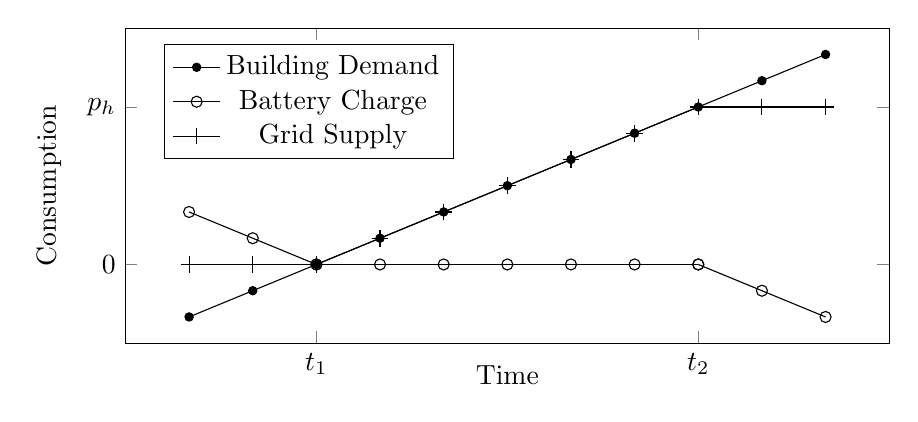
\begin{tikzpicture}

\begin{axis}[
width=0.8\columnwidth,height=4cm,scale only axis,
axis line style={-}, xtick style={-}, ytick style={-},
xlabel=Time,
ylabel=Consumption,
every axis y label/.style={at={(-0.1,0.5)},rotate=90,anchor=center}, 
every axis x label/.style={at={(0.5,-0.1)},anchor=center}, 
%grid=both, grid style={style=densely dotted},
xtick={2,8},
xticklabels={$t_1$,$t_2$},
ytick={0,6},
yticklabels={$0$,$p_h$},
legend style={at={(0.05,0.95)},anchor=north west}
] 

% Draw the Demand-Supply curve
\addplot[-,mark=*,mark size=1.5] expression[domain=0:10,samples=11] {x-2};
\addlegendentry{Building Demand} 

% Draw the Battery curve
\addplot[-,mark=o,mark size=2] expression[forget plot,domain=0:2,samples=3] {2-x}; 
\addplot[-,mark=o,mark size=2] expression[forget plot,domain=2:8,samples=7] {0}; 
\addplot[-,mark=o,mark size=2] expression[domain=8:10,samples=3] {8-x}; 
\addlegendentry{Battery Charge} 

% Draw the Grid supply curve
\addplot[-,mark=+,mark size=3] expression[forget plot,domain=0:2,samples=3] {0}; 
\addplot[-,mark=+,mark size=3] expression[forget plot,domain=2:8,samples=7] {x-2}; 
\addplot[-,mark=+,mark size=3] expression[domain=8:10,samples=3] {6}; 
\addlegendentry{Grid Supply} 
\end{axis} 
\end{tikzpicture} 

%}
}
\qquad
\subfigure[Goal-plan hierarchy for a $k$-modules battery system.]{\label{fig:gptree}
%\resizebox{0.9\columnwidth}{!}{
%!TEX root = ../aamas11storage.tex
\begin{tikzpicture} [level distance=8.0em]
\tikzstyle{planbox}=[draw,text width=11.0em,rectangle split,rectangle split parts=3]
\tikzstyle{goalbox}=[draw,rounded corners=1.25em,minimum height=3em,minimum width=5em]

	
\tikzstyle{level 1}=[sibling distance=13.0em] 
\tikzstyle{level 2}=[level distance=7.0em] 

\node[goalbox,solid] {$G($r,k,s$)$}
	child {node[planbox] {$SetCharge$ 
			\nodepart{second} $\psi:satisfies(r,k,s,C),$\\$k>0$
			\nodepart{third} $set(k,C)$
		}
		child {node[goalbox] {$G($r,k-1,s'$)$}}
	}
	child {node[planbox] {$SetDischarge$ \nodepart{second}
			\nodepart{second} $\psi:satisfies(r,k,s,D),$\\$k>0$
			\nodepart{third} $set(k,D)$
		}
		child {node[goalbox] {$G($r,k-1,s'$)$}}
	}
	child {node[planbox] {$SetNotUsed$ \nodepart{second}
			\nodepart{second} $\psi:satisfies(r,k,s,N),$\\$k>0$
			\nodepart{third} $set(k,N)$
		}
		child {node[goalbox] {$G($r,k-1,s'$)$}}
	}
	child {node[planbox] {$Execute$ 
			\nodepart{second} $\psi:k==0$
			\nodepart{third} $operate()$ \\$evaluate()$
		}
	}
;

\end{tikzpicture}



%}
}
\caption{An energy storage application.}
\end{center}
\label{fig:energystorage}
\end{figure*}


% \newcommand{\aSet}{\mathname{set}}
% \newcommand{\aOperate}{\mathname{operate}}
% \newcommand{\aEvaluate}{\mathname{evaluate}}
% 
% \newcommand{\pSet}{\mathname{Set*}}
% \newcommand{\pSetCharge}{\mathname{SetCharge}}
% \newcommand{\pSetDischarge}{\mathname{SetDischarge}}
% \newcommand{\pSetNotUsed}{\mathname{SetNotUsed}}
% \newcommand{\pExecute}{\mathname{Execute}}
% 
% \newcommand{\cSatisfies}{\psi}
% 
% \begin{figure*}[t]
% \begin{center}
% \subfigure[Use case scenario for a modular battery system.]{\label{fig:usecase}
% %\resizebox{0.9\columnwidth}{!}{
% %!TEX root = ../aamas11storage.tex
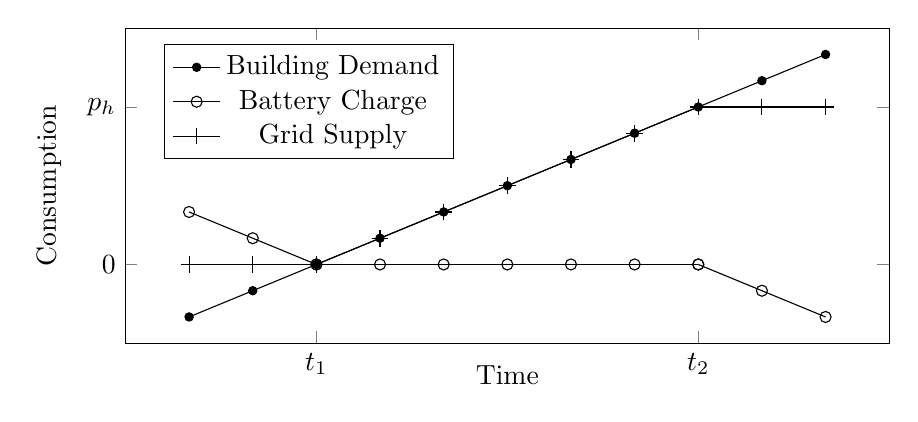
\begin{tikzpicture}

\begin{axis}[
width=0.8\columnwidth,height=4cm,scale only axis,
axis line style={-}, xtick style={-}, ytick style={-},
xlabel=Time,
ylabel=Consumption,
every axis y label/.style={at={(-0.1,0.5)},rotate=90,anchor=center}, 
every axis x label/.style={at={(0.5,-0.1)},anchor=center}, 
%grid=both, grid style={style=densely dotted},
xtick={2,8},
xticklabels={$t_1$,$t_2$},
ytick={0,6},
yticklabels={$0$,$p_h$},
legend style={at={(0.05,0.95)},anchor=north west}
] 

% Draw the Demand-Supply curve
\addplot[-,mark=*,mark size=1.5] expression[domain=0:10,samples=11] {x-2};
\addlegendentry{Building Demand} 

% Draw the Battery curve
\addplot[-,mark=o,mark size=2] expression[forget plot,domain=0:2,samples=3] {2-x}; 
\addplot[-,mark=o,mark size=2] expression[forget plot,domain=2:8,samples=7] {0}; 
\addplot[-,mark=o,mark size=2] expression[domain=8:10,samples=3] {8-x}; 
\addlegendentry{Battery Charge} 

% Draw the Grid supply curve
\addplot[-,mark=+,mark size=3] expression[forget plot,domain=0:2,samples=3] {0}; 
\addplot[-,mark=+,mark size=3] expression[forget plot,domain=2:8,samples=7] {x-2}; 
\addplot[-,mark=+,mark size=3] expression[domain=8:10,samples=3] {6}; 
\addlegendentry{Grid Supply} 
\end{axis} 
\end{tikzpicture} 

% %}
% }
% \qquad
% \subfigure[Goal-plan hierarchy for a $k$-modules battery system.]{\label{fig:gptree}
% %\resizebox{0.9\columnwidth}{!}{
% %!TEX root = ../aamas11storage.tex
\begin{tikzpicture} [level distance=8.0em]
\tikzstyle{planbox}=[draw,text width=11.0em,rectangle split,rectangle split parts=3]
\tikzstyle{goalbox}=[draw,rounded corners=1.25em,minimum height=3em,minimum width=5em]

	
\tikzstyle{level 1}=[sibling distance=13.0em] 
\tikzstyle{level 2}=[level distance=7.0em] 

\node[goalbox,solid] {$G($r,k,s$)$}
	child {node[planbox] {$SetCharge$ 
			\nodepart{second} $\psi:satisfies(r,k,s,C),$\\$k>0$
			\nodepart{third} $set(k,C)$
		}
		child {node[goalbox] {$G($r,k-1,s'$)$}}
	}
	child {node[planbox] {$SetDischarge$ \nodepart{second}
			\nodepart{second} $\psi:satisfies(r,k,s,D),$\\$k>0$
			\nodepart{third} $set(k,D)$
		}
		child {node[goalbox] {$G($r,k-1,s'$)$}}
	}
	child {node[planbox] {$SetNotUsed$ \nodepart{second}
			\nodepart{second} $\psi:satisfies(r,k,s,N),$\\$k>0$
			\nodepart{third} $set(k,N)$
		}
		child {node[goalbox] {$G($r,k-1,s'$)$}}
	}
	child {node[planbox] {$Execute$ 
			\nodepart{second} $\psi:k==0$
			\nodepart{third} $operate()$ \\$evaluate()$
		}
	}
;

\end{tikzpicture}



% %}
% }
% \caption{An energy storage application.}
% \end{center}
% \label{fig:energystorage}
% \end{figure*}


The confidence measure $\C_s$ would make a useful heuristic for exploration (i.e., plan selection) in its own right: such that when the confidence is at its lowest we do maximum exploration and when it is at its highest we fully utilise the decision tree. The problem with this approach, however, is that $\C_s$ only covers the space of known worlds. This means that whenever a new world is witnessed, $\C_s=0.0$, meaning that we will choose randomly. This is hardly beneficial since what we would really like is to use the learnt generalisations to classify this new world rather than be agnostic about it. What is missing is a metric that contributes to our net confidence but that is independent of $w$.

One way to achieve this is by monitoring the rate at which new worlds are being witnessed by the plan $P$. During early exploration it is expected that the majority of worlds that a plan is selected for will be unique, therefore this rate is high and our confidence is low. Over time as exploration continues, the plan would get selected in all possible worlds and the rate of new worlds would approach zero while our confidence over this period would increase to its maximum.  Equation \ref{eqn:confidence-domain} defines this confidence metric $\C_d$ for plan $P$ over the last $n$ executions. Here, $W(P,*)$ is the set of all worlds witnessed by $P$ since the beginning and $\triangle W(P,n)$ is the set of worlds witnessed in the last $n$ executions. $\C_d$ is guaranteed to converge to $1.0$ as long as all worlds where the plan might apply are eventually witnessed.

\begin{equation}
\C_d(P,n) = \frac{|W(P,*)\cap \triangle W(P,n) |}{n}.
\label{eqn:confidence-domain}
\end{equation}

We are now ready to define our final confidence measure $\C$ based on the two component confidence metrics $\C_s$ and $\C_d$. Equation \ref{eqn:confidence} describes this calculation. Here $\alpha$ is the weighting factor used to set a preference bias between the two components.

\begin{equation}
\C(P,w,n) = (\C_s(P,w,n)*\alpha) + [\C_d(P,n)*(1.0-\alpha)].
\label{eqn:confidence}
\end{equation}

Finally, Equation \ref{eqn:omega} shows how the confidence measure $\C$ is used as a exploration heuristic during plan selection. Here $\P$ is the probability of success of plan $P$ in world $w$ as given by its decision tree and $\Omega$ is the plan selection weight. This formulation of the plan selection weight is similar to those presented in \cite{singh10:extending, singh10:learning} bar the replacement of earlier measures with the new confidence term $\C$.

\begin{equation}
\Omega(P,w,n) = 0.5 + \left[  \C(P,w,n) *  \left( \P(P,w) - 0.5 \right)  \right]
\label{eqn:omega}   
\end{equation}

The storage domain scenario (c.f. Section \ref{sec:application}) highlights the benefits of our dynamic confidence measure of Equation \ref{eqn:confidence}. In this domain it is easy to think of situations where the dynamics of the environment changes such that the solution space varies over time. For instance, our motivation for learning is that battery chemistry (and therefore performance) deteriorates over time, and the system should learn to avoid solutions that no longer work in the future. However, worn battery modules get replaced every now and then, and hence, some configurations that the learner may have eliminated previously may become applicable once again. Similar examples may be conjured for situations involving module malfunctions. The point is that each such change in the environment impacts the solution space in some way, however an explicit notification, that may be used to trigger a change in behaviour, is not always available (some changes may be continuous, for instance). Moreover, several such factors may play on the solution space at one time, and it is up to the learner to respond in this environment appropriately.


Here it becomes important for an agent to reliably recognise such changes, and respond by adjusting its exploration strategy accordingly (or perhaps, switching policies, choosing to learn afresh, and so on). Since the new confidence measure is built using observed data alone, it consequently reflects agent performance: our confidence is maximum when the rate of change in observed performance and worlds states is stable, and minimum when it is not. Importantly, this means that the measure is non-monotonic and as such may be used to dynamically tune the exploration strategy (for instance during plan selection as in Equation \ref{eqn:omega}) against a variable solution space.
